\documentclass{llncs}

\usepackage{llncsdoc}
\usepackage[utf8]{inputenc}
\usepackage{graphicx}
\usepackage[spanish]{babel}
\usepackage[margin=3cm]{geometry}
\usepackage{hyperref}
\usepackage{listings}

%META INFO DEL DOCUMENTO

%% TITULO
\title{Battle-sim: Simulador de enfrentamientos bélicos}
%% AUTORES
\author{Rocio Ortiz Gancedo - C311\\Carlos Toledo Silva - C311\\Ariel A. Triana Pérez - C311}
\date{2022}

\pagenumbering{gobble}
\begin{document}

\markboth{Battle-sim: Simulador de enfrentamientos bélicos}{Battle-sim: Simulador de enfrentamientos bélicos}
\thispagestyle{empty}


\makeatletter

    % PORTADA DEL DOCUMENTO %
    \begin{titlepage}
        \centering
        
        
\includegraphics[width=0.2\textwidth]{chapters/img/logo-matcom.jpg}
        
        \vspace{0.5cm}
        
        {\scshape \LARGE Universidad de La Habana \par}
        {\scshape \Large Facultad de Matemática y Computación \par}
        
        \vspace{6.5cm}
        
        {\bfseries \Huge \textbf{\@title} \par}
        \vspace{0.2cm}
        \textit{Proyecto de Inteligencia Artificial, Compilación y Simulación}
        
        \vfill
        
        \textbf{Equipo de desarrollo:}
        
        \@author
        
        \vspace{1cm}
        
        \@date
    \end{titlepage}
    % FIN DE LA PORTADA %

    % INDICE %
    \tableofcontents
    % FIN DEL INDICE %

    % CAPITULOS %
    \mainmatter
    \section{Introducci\'on}

A lo largo de la historia, los conflictos b\'elicos han estado fuertemente ligados al desarrollo de la humanidad. Existen pruebas que desde la prehistoria, los hombres luchaban entre ellos por tierras y recursos naturales. Con el pasar del tiempo, los hombres fueron evolucionando, y as\'i tambi\'en lo hicieron los objetivos de los conflictos b\'elicos, los armamentos y estrategias utilizados en estos conflictos.

El objetivo de este proyecto es el desarrollo de un programa que permita la simulaci\'on de diferentes batallas que se hayan producido en un pasado distante, en \'epocas m\'as recientes e incluso simular batallas futuristas o con elementos de fantas\'ia. Adem\'as se podr\'ian simular batallas entre diferentes \'epocas, por ejemplo podr\'iamos enfrentar 300 soldados armados con las m\'as modernas armas contra 1000 soldados armados con espadas y escudos. 
    \section{La Simulaci\'on}

Como planteamos en el cap\'itulo anterior, se quiere desarrollar un programa que permita la simulaci\'on de enfrentamientos b\'elicos entre dos o m\'as bandos.

Para esto se tienen pensado los siguientes aspectos que van a ser fijos en cada una de las simulaciones:

\begin{enumerate}
	\item La existencia de un mapa o terreno donde se producir\'a el enfrentamiento. Este tendr\'a propiedades que se ser\'an modificables como las dimensiones, el relieve, la hidrograf\'ia, etc. La idea es que este se represente por una matriz bidimensional.
	
	\item Las acciones ser\'an por turnos. Como tenemos dos bandos les llamaremos: bando A y bando B. En el turno del bando A cada una de las unidades de A realizar\'a una y solo una acci\'on (ya sea moverse hacia otra posici\'on, atacar o mantener la posici\'on). Luego de esto se pasar\'a al turno del bando B, que al igual que A, podr\'a hacer una y solo una acci\'on con cada una de sus unidades. Esta forma de implementaci\'on permite un comportamiento de acci\'on-reacci\'on entre los dos bandos, asemej\'andose a lo que ocurre en la vida real.
	
\end{enumerate}

\subsection{El mapa}

El mapa consiste en una matriz bidimensional de $m$ filas y $n$ columnas. Cada objeto de la matriz es un objeto \verb|Cell|. Un objeto \verb|Cell| representa cada una de las casillas que conforman el mapa y tiene los siguientes atributos:

\begin{itemize}
	\item \verb|passable|: Valor entre 0 y 10 que indica cuan accesible es una celda. Las unidades tienden a buscar las celdas que tengan este par\'ametro lo m\'as alto posible, pues mientras mayor sea este valor, pueden hacer ataques m\'as poderosos.
	\item \verb|row|: Este par\'ametro es un n\'umero entero que indica la fila en la que se encuentra la celda.
	\item \verb|col|: Este par\'ametro es un n\'umero entero que indica la columna en que se encuentra la celda
	\item \verb|height|: Este par\'ametro es un n\'umero entre 0 y 1 que indica la altura de la casilla. En dependencia de este par\'ametro la casilla ser\'a terrestre o marina.
	\item \verb|bs_object|: Este par\'ametro hace referencia al objeto que se encuentra en la casilla. Si en la casilla no se encuentra ning\'un objeto entonces este par\'ametro es \verb|None|.
\end{itemize}

El mapa para una simulaci\'on se crea instanciando una clase \verb|LandMap| con los siguientes argumentos:

\begin{itemize}
	\item N\'umero de filas $m$
	\item N\'umero de columnas $n$
	\item Un array bidimensional de $m$ filas por $n$ columnas tal que cada posici\'on $i,j$ del array es un n\'umero entre 0 y 10 que indica cuan accesible es la celda $i,j$
	\item Un array bidimensional de $m$ filas por $n$ columnas tal que cada posici\'on $i,j$ del array es un n\'umero entre 0 y 1 que indica la altura de celda $i,j$
	\item Un n\'umero entre 0 y 1 que indica el nivel del mar. Todas las celdas cuya altura sea menor a este n\'umero ser\'an consideradas como celdas marinas y todas las celdas superior a este n\'umero ser\'an consideradas terrestres.
\end{itemize}

\subsubsection{Generación aleatoria de mapas}

La representación abstracta de un mapa es una matriz de alturas, o sea, una matriz de valores en el intervalo $[0,1]$, donde la noción de nivel del mar es 0.45, o sea, todo valor $x > 0.45$ es una elevación y todo valor $x < 0.45$ es una depresión cubierta por agua. Es importante poder generar un mapa de alturas con un porcentaje de relieve determinado por el usuario que sea lo más realista posible pero esto de forma aleatoria. Por tal razón queda totalmente descartado el enfoque que va por generar una matriz $M$ donde $M[i,j]$ es un número totalmente al azar, pues se obtendrían matrices de ruido similares a la estática en las señales de televisión, además se violaría la restricción del porciento de elevaciones.

\begin{figure}
	\centering
	
\includegraphics[width=8cm]{chapters/img/estatica.jpg}
	\caption{Estática en la señal de TV}
\end{figure}

Luego de una consulta bibliográfica, se encontraron algunos procedimientos para la generación de mapas de alturas muy interesantes:

\begin{itemize}
	\item \textbf{Algoritmo de Perlin Noise:} debe su nombre a su creador, Ken Perlin, que durante el rodaje de la película Tron creó el algoritmo con el fin de crear texturas procedimentales para los efectos generados por el ordenador. La idea tras el algoritmo es generar una nueva matriz de dimensión menor a la requerida y superponerla a la requerida escalando de forma que encajen perfectamente. A cada esquina de cada celda de la nueva matriz se le asigna un vector gradiente pseudoaleatorio. Además se determinan los valores offset que representan la posición de cada punto de la matriz original dentro de la celda de la nueva matriz. Luego, para cada esquina de la celda que encierra un punto se determina el vector que va desde ella hasta el punto y se hace el producto escalar de ese vector con el vector gradiente. Se realiza una interpolación lineal entre todos los resultados de los productos escalares y este es el valor del punto. El comportamiento de este algoritmo no puede ser modificado pero aún así fue de gran significación en la época y hoy día.
	\item \textbf{Algoritmo Voronoi:} consiste en dividir el espacio en diagramas de Voronoi, que son, simplemente, particiones de un plano en regiones basadas en la 	distancia a ciertos puntos específicos del plano. Ese conjunto específico de puntos 	se denomina ``semillas, sitios o generadores''. Se suelen especificar de antemano y 	para cada uno de estos sitios se genera una región del plano que consiste en todos 	los puntos que están más cerca de este sitio que de ningún otro. 
	\item \textbf{Algoritmo de cortes:} tiene un comportamiento poco intuito pero interesante, se selecciona un corte en la matriz, se define como corte una linea recta que divida el plano o terreno en dos mitades, luego se decide elevar  una de las mitades y bajar o no modificar las otras. Este mismo proceso se repite miles de veces y se obtienen resultados aceptables. El algoritmo es ineficiente, por la cantidad de iteraciones necesarias para obtener buenos resultados.
	\item \textbf{Algoritmos de erosión térmica e hídrica:} algoritmos que simulan los procesos naturales de erosión térmica e hídrica. En el caso de la térmica se fija un valor $T$ que representa el valor a partir del cual se va a erosionar, y se recorre la matriz buscando los puntos que cumplen que la diferencia de altura con sus vecinos es superior a $T$. En dichos puntos el algoritmo resta valor de altura a sus vecinos cuya distancia sea mayor que $T$ de forma que todas las distancias queden menor que $T$. En el caso de la erosión hídrica se define una matriz de agua y una matriz de sedimentos la cual representa un porciento de material que puede ser movido por la erosión. Y se realiza un procedimiento parecido a la erosión térmica.
\end{itemize}

Ahora estos algoritmo generan mapas de alturas con apariencia realista, pero no son suficientes para cumplir las restricciones de relieve. Por tanto, nuestra propuesta es la implementación de un algoritmo evolutivo que genera un mapa de alturas realista y satisfaga la restricción anteriormente mencionada.

Los algoritmos evolutivos son estrategias de optimización y búsqueda de soluciones que toman como inspiración la evolución en distintos sistemas biológicos. La idea fundamental de estos algoritmos es mantener un conjunto de individuos que representan una posible solución del problema. Estos individuos se mezclan y compiten entre sí, siguiendo el principio de selección natural por el cual sólo los mejor adaptados sobreviven al paso del tiempo. Esto redunda en una evolución hacia soluciones cada vez más aptas. 

El algoritmo evolutivo en cuestión inicia con una población de individuos generados utilizando el algoritmo de Perlin Noise implementado en la biblioteca de Python bajo el nombre \verb|perlin-noise|.	Luego se realizan un cantidad de iteraciones seleccionando los individuos más adaptados, mezclándolos y mutándolos.  Se considera individuo mejor adaptado aquel cuyo valor \verb|fit| sea mayor. Este valor se calcula como sigue:

\begin{verbatim}
def fit_func(self, heightmap: HeightMap):
	count = sum(sum(heightmap.__map__ > self.__sea__))
	per = count / prod(self.__shape__)
	return per if per < self.percentage else 0
\end{verbatim}
\subsection{Los objetos}

Un objeto es todo lo que se puede poner el mapa y cada objeto ocupa una y solo una casilla del mapa. Estos tienen propiedades como el id que s \'unico para cada objeto, los puntos de vida que determinan el estado de un objeto y la defensa un par\'ametro que indica cuan resistente es un objeto a los da\~{n}os que puede sufrir durante la simulaci\'on. Todos estos par\'ametros son n\'umeros de 1 a 10. Cuando la vida de un objeto llegue a 0, este se destruye desapareciendo del mapa. Los objetos se clasifican en dos tipos: unidades y objetos est\'aticos. Los objetos adem\'as tienen definidas dos funciones \verb|put_in_cell| cuya funci\'on es colocar al objeto en alguna posici\'on de un mapa. Si se intenta poner un objeto en una posici\'on diferente a su tipo este autom\'aticamente se destruye. La otra funci\'on \verb|take_damage|, a partir de un ataque sufrido indica como se reducen los puntos de vida del objeto.

\subsubsection{Objetos est\'aticos}

Los objetos est\'aticos los podemos definir como objetos propios del ambiente. Estos no pertenecen a ning\'un bando y no pueden realizar acciones pero si pueden ser afectados por las acciones que realicen las unidades. Estos solo pueden ser puestos en celdas terrestres. Ejemplos de estos objetos pueden ser \'arboles, rocas, muros, etc. Todos estos objetos son terrestres. 

\subsubsection{Unidades}

Las unidades son los agentes de la simulaci\'on. El objetivo de cada una de las unidades es destruir a las unidades enemigas (las que no pertenecen a su mismo bando), y para ello podr\'a analizar parte del ambiente en el que se encuentra y tomar la decisi\'on que sea m\'as conveniente seg\'un sean las circunstancias. 

Dado que el ambiente estar\'a cambiando constantemente, las unidades ser\'an agentes casi puramente reactivos. La arquitectura empleada para definir el comportamiento de las unidades es la Arquitectura de Brooks (de categorización o inclusión) que recordemos tiene las siguientes caracter\'isticas: 

\begin{itemize}
	\item La toma de decisión se realiza a través de un conjunto de comportamientos para lograr objetivos (reglas de la forma situación $\rightarrow$ acción).
	\item Las reglas pueden dispararse de manera simultánea por lo que debe un mecanismo para escoger entre ellas.	
\end{itemize}

Dado esto se defini\'o un sistema experto que actuar\'a como la funci\'on del agente. Este ser\'a descrito posteriormente.

\textbf{Propiedades de las unidades}

Las unidades adem\'as de las descritas anteriormente que tienen todos los objetos cuentan con las siguientes propiedades:

\begin{itemize}
	\item \verb|side|: Una instancia de la clase \verb|Side| que indica el bando al que pertenece la unidad
	\item \verb|attack|: Valor entre 1 y 10 que marca la capacidad de causar da\~{n}os a sus oponentes.
	\item \verb|moral|: Valor entre 1 y 10 que marca la moral con la unidad encara la batalla. Cuanto mayor es ese valor m\'as efectivos son sus ataques y sus defensas.
	\item \verb|ofensive|: Valor entre 1 y 10 que indica cuan ofensiva es una unidad. Un valor alto la hace m\'as ofensiva y un valor bajo la hace m\'as defensiva.
	\item \verb|min_range|: Valor entero entre 0 y 10 que indica el rango m\'inimo al que se debe encontrar un enemigo para que la unidad pueda atacarlo.
	\item \verb|max_range|: Valor entero entre 0 y 10 que indica el rango m\'aximo al que se debe encontrar un enemigo para que la unidad pueda atacarlo.
	\item \verb|radio|: Valor entero entre 1 y 9 que indica el n\'umero de casillas que son afectadas por un ataque de la unidad. Si es 1 se afecta solo a la casilla seleccionada para el ataque. Si es 9 se afectan la casilla seleccionada y las 8 adyacentes a esta. Si es 1 $<$ \verb|radio| $<$ 9, entonces se toman como casillas afectadas la seleccionada y $\verb|radio|-1$ casillas adyacentes a esta.
	\item \verb|vision| : Valor entre 1 y 10 que indica la cantidad de celdas en una determinada direcci\'on, que la unidad puede ``ver'' (saber que objetos est\'an en dicha celda).   
	\item \verb|intelligence|: Valor entre 0 y 10 que indica la inteligencia de la unidad. Mientras m\'as inteligente sea una unidad con mayor precisi\'on puede calcular los atributos de sus enemigos.
	\item \verb|recharge_turns|: Turnos que demora la unidad en recargar despu\'es de hacer un ataque. Mientras est\'e recargando la unidad no podr\'a atacar pero si puede moverse.
	\item \verb|solidarity|: Valor booleano que indica si la unidad es solidaria o no.
	\item \verb|movil|: Valor booleano que indica si la unidad puede desplazarse por el mapa.  
\end{itemize}

\subsubsection{Sistema experto}

A continuaci\'on se explicar\'a el sistema experto implementado que act\'ua como funci\'on del agente la cual describe el comportamiento del agente durante un turno.


Lo primero que la funci\'on hace es buscar si se existe un enemigo al que se pueda atacar. Para eso primero se comprueba si la unidad no est\'a recargando, si lo est\'a se reduce en uno los turnos que debe esperar para atacar, si no lo est\'a se busca el mejor enemigo para atacar. 
 
El mejor enemigo para atacar se determina de la siguiente forma:
 
Por cada casilla atacable (casilla que se encuentra a una distancia de la unidad entre su rango m\'inimo y su rango m\'aximo), se chequea si en la casilla hay un enemigo. Si el radio de ataque es mayor que 1 y hay una unidad amiga cerca del enemigo que pudiera verse afectada por el ataque, se ignora este enemigo. Esto se defini\'o as\'i para evitar el da\~{n}o ocasionado por fuego amigo.
 
Entonces si el enemigo no es ignorado debido a lo anterior, se calcula el costo de atacar al enemigo. Para dicho c\'alculo la unidad estima la vida y la defensa del enemigo y con estas estimaciones calcula cuantos turnos podr\'ia tomarle destruir a dicho enemigo. Mientras mayor sea la inteligencia de la unidad m\'as precisas ser\'an las estimaciones.

Luego de haber analizado todos los enemigos, el seleccionado por la unidad para atacarlo es aquel cuyo costo es menor. Si no se detecta ning\'un posible enemigo a atacar entonces la unidad no realiza un ataque en el turno.
 
Si la unidad no realiza un ataque, entonces, en caso de que se m\'ovil, chequea si se puede mover a alguna casilla adyacente a la que se encuentra. Esto se hace de la siguiente forma:
 
Se fija un costo en infinito. Luego por cada una de las celdas que la rodean en todos los puntos cardinales posibles (NW, N, NE, W, E, SW, S y SE)ase calcula el costo de moverse a dicha celda, y nos quedamos con la celda cuyo co es el menor. Luego si el menor costo detectado es menor a infinito la unidad se mueve a dicha celda en caso contrario la unidad mantiene su posici\'on. 
 
Ahora veamos como calcular el costo de que una unidad se mueva de una celda a otra.
 
Si la celda nueva es intransitable (tiene el par\'ametro \verb|passable| en 0), el tipo de la celda es diferente al tipo de la unidad o si en la celda hay alg\'un objeto se devuelve infinito. Estos son todos los casos en los que la unidad no puede moverse a dicha celda. Para las unidades terrestres siola diferencia de alturas entre dosla ltas es muy grande (mayor a 0.3), tampoco pueden avanzar a dicha celda, retorn\'andose infinito. 
 
Entonces en un primer momento se fija el costo en 10 - \verb|passable|/2, de esta manera se premia ir a celdas m\'as transitables. A continuaci\'on se comprueba si esa celda est\'a entre las que la unidad recuerda como ya visitadas. Si as\'i es, el coste se incrementar\'a en \verb|passable|/3. As\'i logramos incentivar que las unidades visiten celdas no visitadas con anterioridad  
  
Ahora se comprueba si la celda se encuentra en zona ``amiga'', es decir, si esa celda es adyacente a alguna celda en la que se encuentre alg\'un compa\~{n}ero de su bando. Si as\'i es y nuestra unidad protagonista es solidaria, el coste se reducir\'a a la mitad. Si es una zona amiga pero la unidad no es solidaria, el coste solo se reducir\'a dividi\'endose por la ra\'iz cuadrada de 2. De esta manera se incentiva que las unidades tiendan a permanecer en grupo y m\'as cuanto m\'as solidarias son.

Si la celda que se est\'a estudiando es una celda en la que nuestra unidad tendr\'a al alcance un enemigo, su coste se reducir\'a en el valor del par\'ametro \verb|ofensive|  multiplicado por la inversa de la ra\'iz cuadrada de la distancia m\'inima hasta el enemigo. Adem\'as la unidad observa las celdas cercanas a la celda que se est\'a estudiando que est\'en dentro de su rango de visi\'on. Si detecta que al moverse a dicha celda se encontrar\'a en rango de alg\'un enemigo el costo se aumenta en 1.1 por cada enemigo que pudiera atacar a la unidad. De esta manera se est\'a diciendo que, cuanto m\'as ofensiva sea nuestra unidad, m\'as se aproximar\'a al enemigo, aunque con cierta precauci\'on.  

\subsection{El simulador}

\subsubsection{Los bandos}

Dentro de la simulaci\'on de batalla las diferentes unidades de los ej\'ercitos  se organizar\'an por bandos que se enfrentar\'an durante la batalla. Dos ej\'ercitos aliados pertenecen al mismo bando y dos ej\'ercitos enemigos pertenecen a bandos distintos.

Para este proceso se implement\'o la clase \verb|Side| que consta de los siguientes atributos y m\'etodos:
\begin{itemize}
\item Atributos
\begin{itemize}
\item \verb|id|: Valor num\'erico \'unico que se le asocia al bando, se utiliza entre otras cosas para hallar el Hash

\item \verb|name|: Nombre que se le dio al bando

\item \verb|units|: Unidades que se encuentran en el bando

\item \verb|no_own_units_defeated|: Cantidad de unidades del bando que fueron derrotadas

\item \verb|no_enemy_units_defeated|: Cantidad de unidades enemigas que han sido derrotadas

\end{itemize}

\item M\'etodos 
\begin{itemize}
\item \verb|add_unit|: Este m\'etodo permite agregar una unidad al bando. Esta acci\'on no tendr\'a efecto hasta el turno siguiente despu\'es de realizarse.

\item \verb|remove_unit|: Este m\'etod posibilita quitar una unidad del bando. Esta acci\'on no tendr\'a efecto hasta el turno siguiente despu\'es de realizarse.

\item \verb|get_units|: Devuelve todas las unidades actuales en la simulaci\'on, aunque estas de momento no realicen turno porque se añadieron recientemente.

\item \verb|__iter__|: Para iterar las unidades

\item \verb|__eq__|: Comparar si dos bandos son el mismo bando

\item \verb|__hash__|: Calcular el hash de un bando
\end{itemize}
\end{itemize}

\subsubsection{Los eventos}

Para la simulaci\'on de la batalla se implement\'o la clase \verb|Simulator|  encargada de simular los eventos que ocurrir\'an durante el enfrentamiento. Se le llamar\'a evento a la acci\'on de alguna de las unidades activas en el terreno en un tiempo determinado, sabiendo que una unidad selecciona la acci\'on a realizar de acuerdo al algoritmo.

La clase \verb|Simulator| consta de los siguientes atributos y m\'etodos:

\begin{itemize}

\item Atributos
 \begin{itemize}
 \item \verb|earth_map|: Mapa del terreno donde ocurre la simulaci\'on
 
 \item \verb|sides|: Bandos que participan en la simulaci\'on
 
 \item \verb|units|: Unidades que participan en la simulación. Incluye a todas las unidades de todos los bandos
 
 \item \verb|time_beg|: Momento en que se empieza la simulaci\'on.
 
 \item \verb|interval|: Tama\~no del intervalo que dura un turno
 
 \item \verb|turns|: Cantidad de turnos a simular.
 
 \item \verb|no_enemies|: Con este atributo se conoce si ya terminó la simulaci\'on, pues almacena si queda m\'as de un bando con unidades vivas.
 
 \end{itemize}
 \item M\'etodos
 
 \begin{itemize}
 \item \verb|event_is_pos|: Revisa si un evento es posible, principalmente comprueba que la unidad que realizar\'a la acci\'on est\'a viva.
 
 \item \verb|get_events|: Toma todas las unidades que a\'un est\'an vivas y les asigna un tiempo de forma aleatoria dentro del intervalo dado. Para seleccionar el tiempo de forma aleatoria se utiliz\'o la distribuci\'on beta que es una distribución de variable aleatoria continua, a diferencia de la uniforme, es bastante m\'as felxible gracias a los par\'ametros $ \alpha $ y $ \beta $, adem\'as de no tener problemas de p\'erdida de memoria como la exponencial. Una vez asociado un tiempo en el que cada unidad viva realizar\'a una acci\'on, estos pasan a ser los eventos a simular.
 
 \item \verb|simulator_by_turns|: Se van a sacar los eventos a partir de un intervalo dado y se ejecutar\'an por orden uno a uno seg\'un el tiempo que se le asign\'o cuando se hizo el evento.
 
 
 \item \verb|simulating_k_turns|: Se sacan los $k$ primeros turnos, a partir del atributo \verb|turns| cada turno en un intervalo de tama\~no \verb|interval|
 \end{itemize}
 
\end{itemize}



    \section{Battle Script, el lenguaje de dominio específico para ejecutar el proyecto}

El usuario final del proyecto necesita un medio para específicar las condiciones del enfrentamiento a simular, entiéndase cómo son las unidades, los soldados, el mapa, el movimiento de las unidades, etcétera. Para ello se implementó un lenguaje de dominio específico (DSL, por sus siglas en inglés \textit{Domain Specific Language}) con el nombre de Battle Script, que permite la creación de nuevas unidades, la creación de obstáculos, la creación de mapas, la inserción de unidades y obstáculos en el mapa, la creación de bandos, y la ejecucción de la simulación.

\subsection{Gramática}

Se diseñó la siguiente gramática para el lenguaje:

\begin{verbatim}
bs_file ->  classes statements EOF     
    |   EOF                       

classes -> class_def  classes         
    |  class_def                       

statements ->   statement  statements      
        |   statement                       

statement ->    func_def
        |   if_def
        |   while_def
        |   decl  ';' 
        |   assign  ';' 
        |   return_stat  ';' 
        |   'break'    ';'                        
        |   'continue'  ';'                       
        |   expressions ;


func_def ->     'function' return_type NAME '(' params ')' '->' block       
        |   'function' return_type NAME '(' ')' '->' block              

if_def ->   'if' expression '->' block elif_def                             
    |   'if' expression '->' block else_def                             
    |   'if' expression '->' block                                      

elif_def ->     'elif' expression '->' block elif_def                       
        |   'elif' expression '->' block else_def                       
        |   'elif' expression '->' block                                

else_def -> 'else' '->' block                                               

class_def ->    'class' NAME 'is' NAME '->' '{'  constructor functions '}'   
    |       'class' NAME 'is' NAME '->' '{'  constructor '}'                     


functions -> func_def  functions                     
       | func_def                                

constructor -> 'constructor' '(' params ')' '->' '{' attributes '}'              
         | 'constructor' '(' ')' '->' '{'  attributes '}'                 
         | 'constructor' '(' ')' '->' '{' '}'                   


attributes -> attr_def  attributes             
        | attr_def                         

attr_def ->  type 'this' '.' NAME '=' expression ';'          


while_def ->    'while' expression '->' block              

return_type ->  'void'                        
        |   type                          

type ->   'number'        
  |   'bool'          
  |   NAME            

assign -> NAME '=' expression                         

decl ->  type NAME '=' expression                              

return_stmt ->  'return' expression                                      
        |   'return'                                        

block ->     '{' statements '}'   

params ->   type NAME ',' params      
    |  type NAME                  


expressions ->  expression ','  expressions               
        |   expression                                

expression ->   disjunction 'if' disjunction 'else' expression            
        |   disjunction                                                

disjunction ->  conjunction 'or' disjunction                                
        | conjunction                                                   

conjunction ->  inversion 'and' conjunction                                 
        |   inversion                                                   

inversion ->    'not' inversion                                             
        |    comparision                                                


comparision ->  sum compare_par                                            
        |   sum

compare_par ->  'eq' sum                        
        |   'neq' sum                       
        |   'lte' sum                       
        |   'lt' sum                        
        |   'gte' sum                       
        |   'gt' sum                        


sum ->  sum '+' term                            
    |   sum '-' term                            
    |   term 

term -> term '*' factor                         
    |   term '/' factor                         
    |   term '%' factor                         
    |   factor

factor ->   '+' factor
    |   '-' factor
    |   pow

pow ->  primary '^' factor              
    |   primary

primary ->  primary '.' NAME            
    |   primary '(' args ')'        
    |   primary '(' ')'             
    |   atom

args -> expression ',' args
    | expression

atom -> NAME                            
    |   'True'                          
    |   'False'                         
    |   'None'                          
    |   NUMBER                          
    |   list

list -> '[' expressions ']'             
    |   '[' ']'                         
\end{verbatim}

\subsection{Compilador}

% TODO: ESCRIBIR MUELA BISCA DEL COMPILADOR
AQUI VA UNA MUELA BISCA DE CóMO ES EL COMPILADOR A GRANDES RASGOS

\subsection{Tokenizador}

Un Tokenizador, comúnmente llamado Lexer, es un ente encargado de dividir la cadena de texto de entrada del compilador en tokens del alfabeto del lenguaje Battle Script, identificando el tipo del token y envíandolo a la siguiente etapa del proceso de compilación.

Para la implementación del tokenizador fue necesario un sistema de expresiones regulares, una clase para representar un token, así como su tipo y la definición de los tokens del lenguaje, además de la clase propia del tokenizador. 

\subsubsection{Sistema de expresiones regulares}

Una expresión regulares es una definición recursiva de un lenguaje donde $a$ es la expresión regular para $L(a) = \{a\}$ y $\epsilon$ es la expresión regular para $L(\epsilon) = \{\epsilon\}$. Si $s$ y $r$ son expresiones regulares entonces:

\begin{itemize}
    \item $(s)|(r)$ es la expresión regular para la unión de lenguajes $L(s) \cup L(r)$
    \item $(s)(r)$ es la expresión regular para la concatenación de lenguajes $L(s)L(r)$
    \item $(s)*$ es la expresión regular para la clausura del lenguaje $L(s)* = \bigcup\limits_{k=0}^{\infty} L(s)^k$
\end{itemize}

Se implementó un sistema de expresiones regulares que admite los siguientes operadores:

\begin{itemize}
    \item $|$ que hace la unión de dos expresiones regulares.
    \item La concatenación de expresiones regulares de la siguiente forma, si $a$ y $b$ son expresiones regulares entonces $ab$ es la expresión de la concatenación.
    \item $*$ que hace la clausura del lenguaje que representa la expresión regular.
    \item $?$ que busca la coincidencia de la expresión regular una vez o ninguna.
    \item $+$ que busca la coincidencia de la expresión regular una o más veces.
    \item $.$ que busca la coincidencia de ninguno o cualquier caracter.
    \item $\setminus$  que permite la inclusión de los operadores anteriores en un expresión regular como un caracter.
\end{itemize}

La gramática para el lenguaje de las expresiones regulares que se implementó es la siguiente:

\begin{verbatim}
    regex = exp 

    exp      = term '|' exp    
            | term

    term     = factor term       
            | factor

    factor   = primary '*'      
            | primary '+'       
            | primary '?'       
            | primary

    primary  = '(' exp ')'
            | '\' CHAR              
            | CHAR
            | '.'
\end{verbatim}

Una expresión regular en el sistema se implementó utilizando la clase \verb|Regex| de Python. Una expresión regular se construye con la cadena de texto que representa el patrón de la expresión regular. Este patrón se compila y se devuelve un Autómata Finito No Determinista (NFA) que se utiliza para los procesos de saber si una cadena pertenece al lenguaje representado por la expresión, o encontrar todas las coincidencias de la expresión en una cadena de texto. 

\begin{verbatim}
class Regex:
        def __init__(self, pattern: str):
            self.pattern : str = pattern
            self.nfa : NFA = self.compile()
    
        def compile(self) -> NFA:
            lex: Lexer = Lexer(self.pattern)
            parser : Parser = Parser(lex)
            tokens : List[Token] = parser()
            handler: Handler = Handler()
            
            nfa_stack : List[NFA]= []
            
            for t in tokens:
                handler.handlers[t.name](t, nfa_stack)
            
            if len(nfa_stack) == 1:
                return nfa_stack.pop() 
            raise Exception("Bad regex!")
    
        def match(self, string: str) -> bool:
            return self.nfa.match(string)
    
        def find_all(self, string: str) -> List[Match]:
            return self.nfa.find_all(string)
\end{verbatim}

El proceso de compilación de una expresión regular es bastante sencillo, se tiene un tokenizador que recorre la cadena y cada vez que encuentra un operador o un caracter devuelve el token correspondiente, si encuentra el operador de escape ($\setminus$) devuelve un token de tipo \verb|CHAR| con el caracter siguiente. El proceso de Parsing consiste en recibir el conjunto de tokens provenientes del tokenizador y llamar al método \verb|exp| que este parsea el no terminal del mismo nombre de la gramática y va parseando el resto de no terminales según corresponda, o sea, se implementó un Parsing Recursivo Descendente.

Luego del proceso de parsing y verificar que la secuencia de tokens es correcta, se recorre la secuencia de tokens y haciendo uso de la clase \verb|Handler| se construye el autómata de la expresión regular. 

La clase \verb|Handler| es la encargada de dado un conjunto de tokens construir el autómata correspondiente, para ello implementa un método para cada operador de la gramática, estos métodos saben construir el autómata que resulta de aplicar la operación a uno, dos o más autómatas según el operador. La clase implementa el algoritmo Thompson's construction para la construcción del 

\begin{itemize}
        \item \textbf{Reconcimiento de un caracter:} el método de la clase \verb|Handler| encargado de construir dicho autómata construye el estado inicial \verb|s0| y el final \verb|s1| y añade la transición con el caracter en cuestión, como se muestra en la figura siguiente:
                \begin{figure}
                        \centering
                        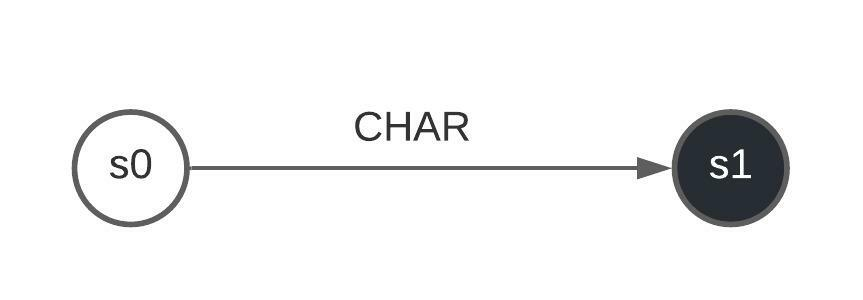
\includegraphics[width=6cm]{./chapters/img/char.jpeg}
                        \caption{Autómata finito no determinista para el reconocimiento de un caracter}
                \end{figure}
        \item \textbf{Operación de Unión:} el método encargado de construir el autómata solo debe los estados iniciales y finales, además añadir $\epsilon$-transiciones desde el estado incial hacia los autómatas y desde los autómatas hacia el estado final.
                \begin{figure}
                        \centering
                        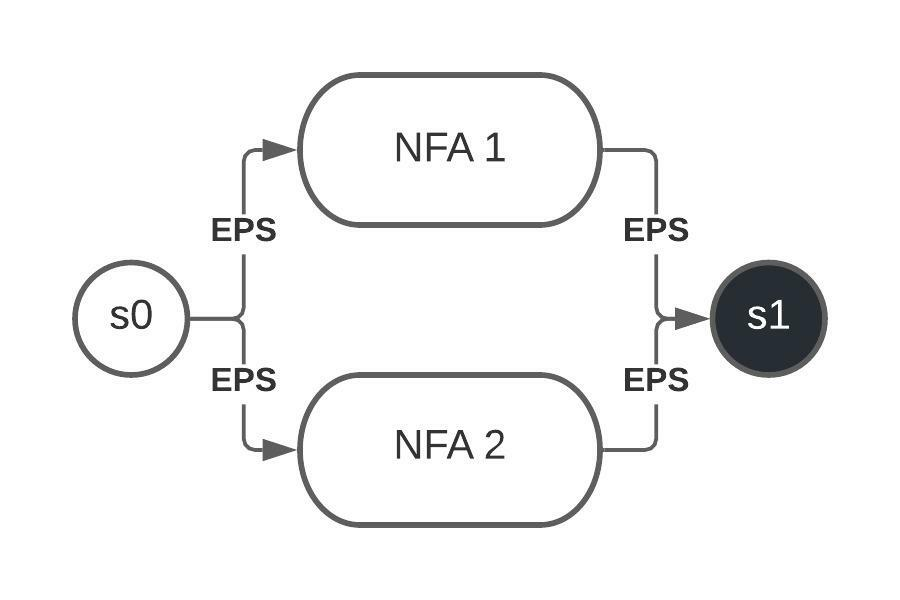
\includegraphics[width=6cm]{./chapters/img/alt.jpeg}
                        \caption{Autómata finito no determinista para el operador unión}
                \end{figure}
        \item \textbf{Operación de Concatenación:} el método encargado de construir el autómata solo debe  añadir una $\epsilon$-transición desde el estado final del primer autómata hacia el estado incial del segundo autómata.
                \begin{figure}
                        \centering
                        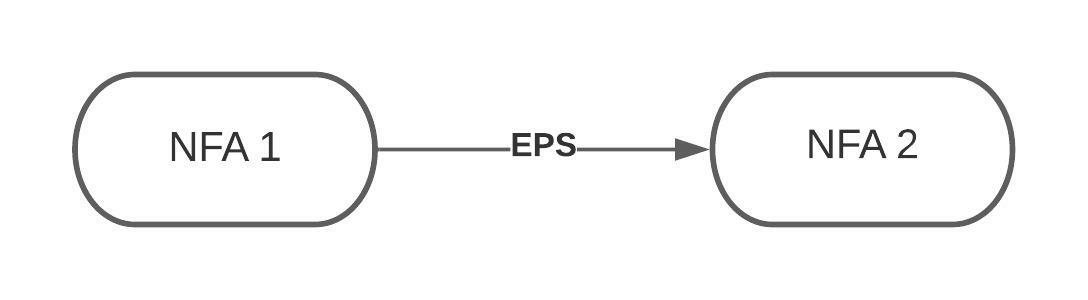
\includegraphics[width=6cm]{./chapters/img/concat.jpeg}
                        \caption{Autómata finito no determinista para el operador concatenación}
                \end{figure}
        \item \textbf{Operación} \verb|*|: el método encargado de construir el autómata solo debe los estados iniciales y finales, además añadir $\epsilon$-transiciones desde el estado incial hacia el autómata y desde el autómata hacia el estado final, así como una desde \verb|s0| hacia \verb|s1| para reconocer la no aparición del patrón, y una transición $\epsilon$ desde el estado final del autómata hacia el inicial para reconocer las repeticiones.
                \begin{figure}
                        \centering
                        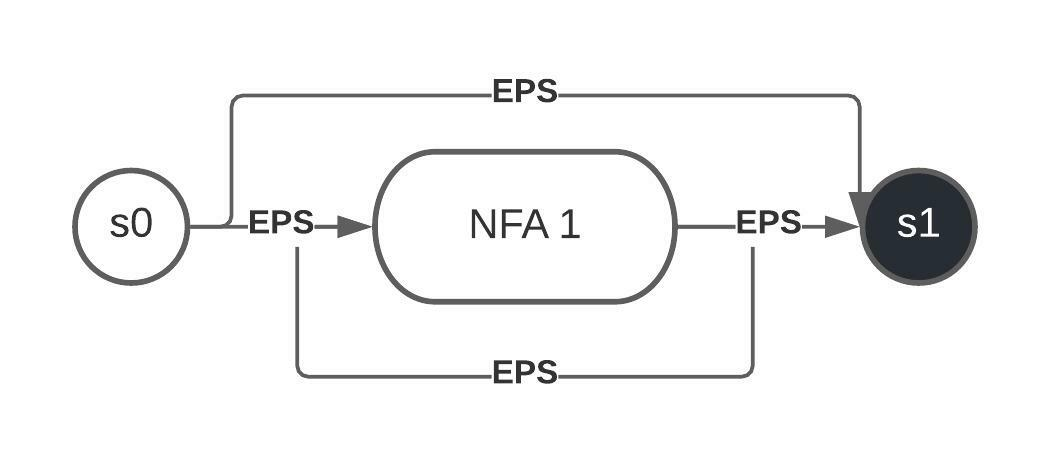
\includegraphics[width=6cm]{./chapters/img/star.jpeg}
                        \caption{Autómata finito no determinista para el operador *}
                \end{figure}
        \item \textbf{Operación} \verb|+|: el método encargado de construir el autómata solo debe los estados iniciales y finales, además añadir $\epsilon$-transiciones desde el estado incial hacia el autómata y desde el autómata hacia el estado final, y una transición $\epsilon$ desde el estado final del autómata hacia el inicial para reconocer las repeticiones.
                \begin{figure}
                        \centering
                        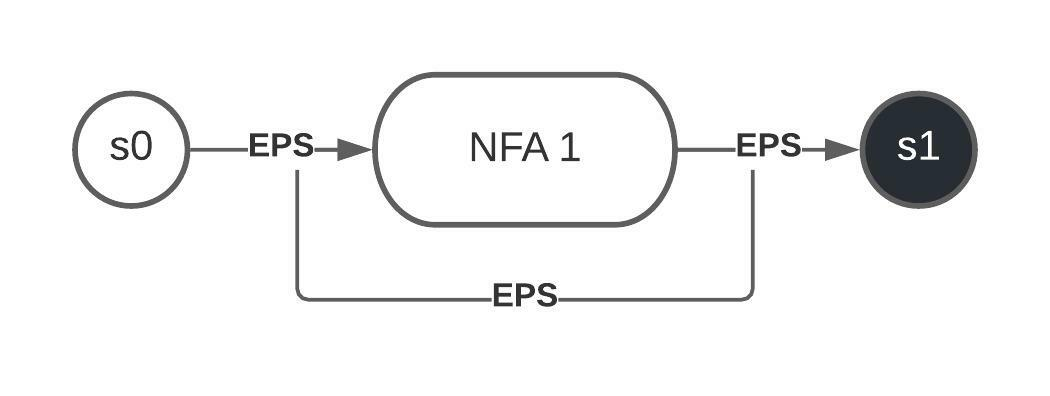
\includegraphics[width=6cm]{./chapters/img/plus.jpeg}
                        \caption{Autómata finito no determinista para el operador +}
                \end{figure}
        \item \textbf{Operación} \verb|.|: el método encargado de construir dicho autómata construye los estados inciales y finales ya añade un transición para cada caracter y añade un $\epsilon$-transición para reconocer la ocurrencia de ningún caracter. El autómata quedaría como el siguiente:
                \begin{figure}
                        \centering
                        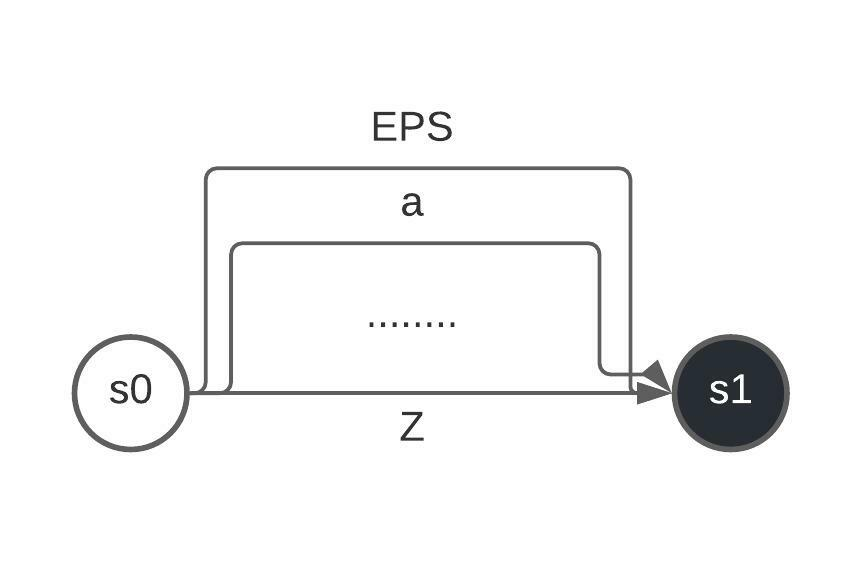
\includegraphics[width=6cm]{./chapters/img/dot.jpeg}
                        \caption{Autómata finito no determinista para el operador .}
                \end{figure}
        \item \textbf{Operación} \verb|?|: el método encargado de construir dicho autómata debe añadir una $\epsilon$-transición desde el estado incial del autómata hacia el estado final del autómata para reconocer la no aparición del patrón.
                \begin{figure}
                        \centering
                        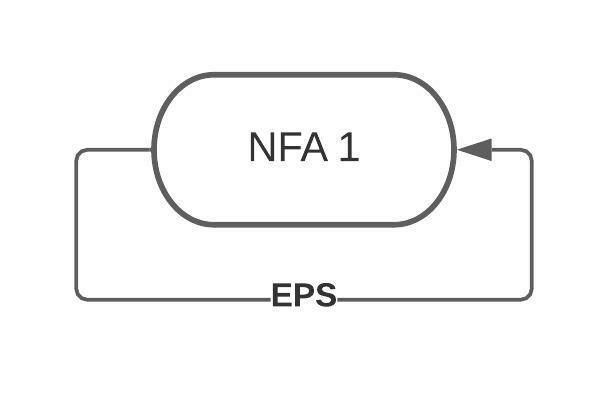
\includegraphics[width=6cm]{./chapters/img/qmark.jpeg}
                        \caption{Autómata finito no determinista para el operador ?}
                \end{figure}
\end{itemize}

Luego que se construye el autómata para una expresión regular  el proceso de compilación ha terminado. 

Entonces, ¿cómo saber si una cadena de texto pertence al alfabeto representado por una expresión regular? Para ello existen varios enfoques entre ellos están:

\begin{itemize}
        \item \textbf{Enfoque inocente o tonto:} utilizando backtracking y revisando los operadores y la cadena. Este enfoque es bien costo y no aprovecha las potencialidades de los autómatas anteriormente construidos.
        \item \textbf{Enfoque DFA:} se construye un Autómata Finito Determinista (DFA) a partir del no determinista anteriormente construido y se hace una pasada sobre él. Este enfoque es correcto, pero implica un procesamiento extra para construir el DFA.
        \item \textbf{Enfoque NFA:} este es el enfoque implementado en el proyecto en el método \verb|match| de una \verb|Regex|, que consiste en hacer una pasada sobre el autómata no determinista y revisar si coincide la cadena, pero el no determinismo trae un problema consigo, es que en un estado \verb|x| no se sabe con total seguridad que transición aplicar. Para ello, la propuesta es ejecutar las transiciones a la vez y ver si por alguna se llega al estado final. Esto hace que el tiempo de reconocimiento sea lineal respecto al tamaño de la cadena de entrada.
\end{itemize}

Entonces, ¿cómo encontrar todas las coincidencias de un patrón dentro de una cadena de texto?. Para ello se modificó el método anterior y cada vez que no se podía continuar  porque venía un caracter desconocido para la expresión regular se volvía al estado inicial. Además en cada posición se revisa si se ha llegado al estado final, se devuelve la coincidencia y se vuelve al estado inicial. Este procedimiento se implementó en método \verb|find_all| de las \verb|Regex|. Este procedimiento es lineal con respecto al tamaño de la cadena.

Luego de implementado el sistema de expresiones regulares se implementó la clase \verb|Token| y el enum \verb|TokenType|.

\subsubsection{Token y TokenType}

Un token en el proyecto se representa con la clase \verb|Token| que tiene la siguiente implementación. La propiedad \verb|regex| almacena la expresión regular que coincide con el token, la propiedad \verb|name| representa el nombre del tipo de token, la propiedad \verb|lexeme| almacena la cadena de texto que se extrajo de la cadena de entrada como token, es decir, si se tiene un token \verb|t| entonces \verb|t.regex.match(t.lexeme)| es verdadero. Además, un token almacena donde comienza y termina \verb|lexeme| en la cadena de entrada.

\begin{verbatim}
class Token:
        @propertyclass Token:
        @property
        def regex(self) -> Regex:
            return self.type.value[0]
    
        @property
        def name(self) -> str:
            return self.type.value[1]
            
        def __init__(self, token_type: TokenType, lexeme: str, start: int, end: int):
            self.type: TokenType = token_type
            self.lexeme: str = lexeme
            self.start: int = start
            self.end: int = end
        
    
        @property
        def name(self) -> str:
            return self.type.value[1]
            
        def __init__(self, token_type: TokenType, lexeme: str, start: int, end: int):
            self.type: TokenType = token_type
            self.lexeme: str = lexeme
            self.start: int = start
            self.end: int = end
        
\end{verbatim}

El tipo de los tokens se definió utilizando el enum \verb|TokenType| que representa la expresión regular que lo representa y el nombre del token, por ejemplo: para el token que representa la palabra reservada \verb|eq| el \verb|TokenType| correspondiente es \verb|Eq = (Regex("eq"), "eq")|

\subsubsection{Algoritmo del tokenizador}

El algoritmo del tokenizador sigue la siguiente idea general, se le asocia a cada token de la gramática un nivel de precedencia que representa cuán relevante es un token sobre otro. Por ejemplo si se tienen los siguientes: \verb|Token((Regex("eq"), "eq"), "eq", 1, 2)| y \texttt{Token((Regex("(a|b|....|Z)+"), "NAME"), 'eq', 1, 2)} donde el primer token tiene precedencia 1 y el segundo tiene 2, entonces el token más relevante es el primero. Entonces, se tiene una lista \verb|tokens| y se recorre la lista de tokens de la gramática y a cada uno se le piden todas coincidencias en la cadena de entrada. Luego se recorren las posiciones \verb|i| de la cadena de entrada, y se añade a \verb|tokens| aquel token que comience en \verb|i| y tenga menor precedencia.

\begin{verbatim}
class Tokenizer:
    def __call__(self, bs_content_file: str) -> Iterable[Token]:
        tokens: List[Token] = []

        matches = {}
        for token_def in TOKENS:
            matches[token_def] = token_def.type.value[0].find_all(bs_content_file)
        
        i = 0
        while i < len(bs_content_file):
            token_in_i: List[Tuple[TokenDefinition, Match]] = []

            # Get all matches
            for k, v in matches.items():
                for t in v:
                    if t.start == i:
                        token_in_i.append((k, t))
                    
            # Get match with highest precedence
            if len(token_in_i):
                token_in_i = sorted(token_in_i, key=lambda tup: tup[0].precendece)
                token = Token(token_in_i[0][0], \
                                token_in_i[0][1].value,\
                                token_in_i[0][1].start,\
                                token_in_i[0][1].end)
                tokens.append(token)    
                i = token.end

            i += 1
        return deque(tokens)
\end{verbatim}

Este algoritmo tiene complejidad temporal $O(n*m)$ donde $m$ es la cantidad de tokens, y $n$ el tamaño de la cadena de entrada.

\subsection{An\'alisis Sem\'antico}
\subsubsection{Definiendo tipos}
Para implementar nuevos tipos en el lenguaje se sigui\'o la idea de Python: se implement\'o una clase \verb|Type| en la que cada clase del lenguaje ser\'a una instancia de esta.
 
  \verb|Type| consta de los siguientes atributos y m\'etodos 
  \begin{itemize}
  \item Atributos
  \begin{itemize}
  \item \verb|name|: Nombre de la clase o nuevo tipo
  
  \item \verb|attributes|: Atributos de la clase.
  
  \item  \verb|methods|: M\'etodos de la clase
  \end{itemize}
  
  \item M\'etodos
  \begin{itemize}
  \item \verb|get_attribute|:  Devuelve el atributo de la clase que se pide si este existe.
  
  \item \verb|get_method|: Devuelve el m\'etodo de la clase que se pide si este existe.
  
  \item \verb|define_attribute|: Define el atriuto de la clase.
  
  \item \verb|define_method|: Define el m\'etodo de la clase.
  
  \item \verb|is_attribute|: Revisa si el atributo existe.
  
  \item \verb|is_method|: Revisa si el m\'etodo existe.
  \end{itemize}
  \end{itemize}
\subsubsection{Context}
Para definir en contexto en el que se escribe un programa con el lenguaje, se implement\'o la clase \verb|Context|, esta cuenta con los siguientes atributos y m\'etodos 
\begin{itemize}
\item Atributos
\begin{itemize}
\item \verb|father|: Contexto padre de este contexto

\item \verb|children|: Contextos hijos de este contexto

\item \verb|_var_context|: Variables del contexto. 

\item \verb|_func_context|: Funciones del contexto

\item \verb|_type_context|: Tipos definidos en el contexto
\end{itemize}

\item M\'etodos
\begin{itemize}
\item \verb|check_var|: Revisa si la variable est\'a definida en el contexto

	\item \verb|check_var_type|: Revisa que la variable est\'e definida en el contexto y el tipo corresponda con el tipo de la variable
	
	\item \verb|check_func|: Revisa que la funci\'on est\'e definida
	
	\item \verb|check_func_args|: Revisa si la funci\'on est\'a definida y los tipos de los argumentos coinciden con los tipos de la funci\'on
	
	\item \verb|get_type|: Devuelve el tipo de una variable en el contexto
	
	\item \verb|define_var|: Si la variable no existe en el contexto, la crea. En caso contrario le asigna el valor siempre que este corresponda con el tipo de la variable
	
	\item \verb|define_func|: Define la funci\'on si no existe en el contexto
	
	\item \verb|create_child_context|: Crea un contexto hijo
	
	\item \verb|create_type|: Crea un nuevo tipo en el contexto
	
	\item \verb|get_return_type|: Dvuelve el tipo de retorno de una funci\'on si esta est\'a definida en el contexto
	
	\item \verb|get_type_object|: Devuelve la clase a la que pertenece objeto dado 
\end{itemize}

\end{itemize}

\subsubsection{Visitor}
Para verificar la correcci\'on de la sem\'antica se implement\'o el patr\'on \verb|Visitor| que visitar\'a el \'arbol de sintaxis abstracta en tres pasadas distintas
\begin{itemize}
\item \verb|Type_Collector|: Es la primera pasada con el patr\'on \verb|Visitor| en este se recogen todos los tipos que se van a definir, para crearlos en el contexto

\item \verb|Type_Builder|: Es la segunda pasada con el patr\'on, se toman todos los tipos que se definieron anteriormente y se definen sus m\'etodos y atributos.

\item \verb|Type_Checker|: Es la tercera pasada con el patr\'on, en esta se revisan que los tipos de cada expresi\'on no entren en contradicci\'on
\end{itemize}
    \section{Ejemplos}

A continuación se muestran algunos ejemplos de uso del compilador y de ejecución de la simulación.

El primer ejemplo que se define a continuación es la creación de la clase Soldier que es un LandUnit. En este caso solo se define el constructor de la clase, que recibe el parámetro \verb|id| que representa el identificador de la unidad en la simulación y el par\'ametro \verb|attack| que es el valor de ataque de la unidad.

\begin{verbatim}
class Soldier is LandUnit -> {  
    constructor(number id, number attack) -> {
        number self.id = id;
        number self.attack = attack;
    };
}; 
\end{verbatim}

Note que tras cualquier instrucción en el lenguaje Battle Script se necesita poner un punto y coma (;) para especificar el fin de la instrucción. En este caso solo se indican los par\'ametros \verb|id| y \verb|attack|. Por tanto el resto de par\'ametros de la unidad tomar\'a los valores por defecto. Dentro de una clase se pueden definir funciones como se muestra en el siguiente ejemplo:

\begin{verbatim}
class Archer is LandUnit -> {
    constructor(number id, number max_range) -> {
        number self.id = id;
        number self.max_range = max_range;
    };
		
    function number plus_id() -> {
        return self.id + 1;
    };
};
\end{verbatim}

En este caso se define una funci\'on que devuelve un n\'umero y no recibe par\'ametros. Obs\'ervese que para hacer referencia a los atributos de la clase se utiliza la palabra clave \verb|self|.

Si se quisiera redefinir una funci\'on  de clase heredada del padre de la clase y en esta utilizar la funci\'on del padre, se puede hacer utilizando la funci\'on super() como se muestra en el siguiente ejemplo:

\begin{verbatim}
    function void turn() -> {
        number a=2*(-1);
        if a lte 1 -> {
            super().turn();
        };
    };
\end{verbatim}

En este caso se ha redefinido la funci\'on \verb|turn|, utilizando adem\'as la funci\'on heredada del padre.

Las definiciones de clases deben ir todas al inicio del programa y cuando se terminen definir todas se debe poner el caracter '\&' para indicar que ya se termin\'o la definici\'on de las clases y ahora se van a comenzar escribir las instrucciones.

Para generar un mapa aleatorio se hace de la siguiente forma:

\begin{verbatim}
	LandMap map = build_random_map(1, 5, 5);
\end{verbatim} 

Entonces pasemos a ver como crear las unidades:

\begin{verbatim}
Soldier sOne = Soldier(1, 10);
Soldier sTwo = Soldier(2, 9);
	
Archer aOne = Archer(3, 5);
Archer aTwo = Archer(4, 5);	
\end{verbatim}  

En este ejemplo hemos creado dos unidades de tipo ``Soldier'' y dos unidades de tipo ``Archer'' utilizando las clases definidas anteriormente.

Para poner una unidad en el mapa se hace de la siguiente forma:

\begin{verbatim}
sOne.put_in_cell(map, 0, 0);
\end{verbatim}

Se toma a la unidad y se hace un llamado a la funci\'on \verb|put_in_cell| pas\'andole como argumentos el mapa y par de enteros que indican la fila y la columna de la celda donde se desea colocar la unidad.

Un bando se crean de la siguiente forma:
  
\begin{verbatim}
Side SOne = Side(1, [sOne, aTwo]);
\end{verbatim}

Como se muestra en los ejemplos anteriores un bando se instancia pas\'andole un id y la lista de unidades que conforman el bando.

Para crear un simulador se hace de la siguiente manera:

\begin{verbatim}
Simulator sim = Simulator(map, [SOne, STwo], 20, 1);
\end{verbatim}

F\'ijese que un simulador se instancia con un mapa, la lista de los bandos, la cantidad de turnos m\'aximos que se desea dure la simulaci\'on y un n\'umero que indica la duraci\'on de un turno.

Para echar andar la simulaci\'on lo hacemos de la siguiente forma: 

\begin{verbatim}
sim.start();
\end{verbatim}

Entonces un ejemplo completo de un programa podr\'ia ser el siguiente:

\begin{verbatim}
class Soldier is LandUnit -> {
    constructor(number id, number attack) -> {
        number self.id = id;
        number self.attack = attack;
    };
};

class Archer is LandUnit -> {
    constructor(number id, number max_range) -> {
        number self.id = id;
        number self.max_range = max_range;
    };
};
&
LandMap map = build_random_map(1, 5, 5);

Soldier sOne = Soldier(1, 10);
Soldier sTwo = Soldier(2, 9);

Archer aOne = Archer(3, 5);
Archer aTwo = Archer(4, 5);

sOne.put_in_cell(map, 0, 0);
aTwo.put_in_cell(map, 0, 1);

aOne.put_in_cell(map, 4,4 );
sTwo.put_in_cell(map, 4, 3);

Side SOne = Side(1, [sOne, aTwo]);
Side STwo = Side(2, [aOne, sTwo]);

Simulator sim = Simulator(map, [SOne, STwo], 20, 1);

sim.start();
	
\end{verbatim}

En el lenguaje adem\'as se pueden definir instrucciones m\'as complicadas tales como: if, while, declaraciones, asignaciones, etc. A continuaci\'on se muestran algunos ejemplos de como hacerlo:

\begin{verbatim}
function number W(number a) -> { 
    if a lt 0 and a eq 0 -> { 
        return -1 * a;  
    } 
    elif a gt 1 -> {
        return 4;
    } 
    else -> { 
        return a; 
    }; 
};

function number A(number a) -> { 
    while a lte 5 -> {
        a = a + 1;
    }; 
    return a;
};
\end{verbatim} 

M\'as ejemplos se pueden encontrar en el m\'odulo test/examples.

    \section{Reflejo de las asignaturas en el proyecto}

\subsection{Simulaci\'on}

Tendr\'iamos como sistema el enfrentamiento b\'elico. Las entidades ser\'ian las unidades, estructuras y elementos del terreno. Como relaciones tendr\'iamos por ejemplo la distancia entre estas entidades, el daño que le causa una unidad a otra, etc. Como proceso tendr\'iamos el movimiento de las unidades, el ataque de una unidad a otra,etc.

Este sistema es observable, permiti\'endonos, al ejecutar simulaciones del mismo, obtener resultados y sacar conclusiones a partir de estos. Es controlable pues las unidades realizan acciones seg\'un estrategias y la simulaci\'on ocurre seg\'un reglas definidas. Es modificable pues podemos agregar y eliminar unidades, adem\'as de cambiar reglas y estrategias, lo que nos permite obtener diferentes resultados.

\subsection{Compilaci\'on}

Se definir\'a un lenguaje en el cual se puedan definir diferentes unidades, estructuras y sus respectivas estad\'isticas, modificar las caracter\'isticas del terreno, crear estrategias y definir reglas para la simulaci\'on.

\subsection{Inteligencia Artificial}
Como las unidades se tendr\'an que mover por el mapa, para lograr un movimiento eficiente de las mismas utilizaremos el algoritmo A*.

Adem\'as como tenemos dos bandos enfrent\'andose nos auxiliaremos de un algoritmo Minimax para realizar los movimientos que har\'an los bandos en sus respectivos turnos, utilizando una heur\'istica basada en la situaci\'on actual del mapa y la estrategia definida por el usuario.

Es muy posible que con el avance de la asignatura y el desarrollo del proyecto utilicemos m\'as herramientas.
    \section{Aplicaciones}

Este proyecto nos permite recrear batallas y estudiar diferentes finales alternativos seg\'un se hubieran comportado diferentes par\'ametros. Adem\'as podemos predecir el desenlace de futuros enfrentamientos y cuales podr\'ian ser las mejores estrategias para que uno u otro bando saliese victorioso, adem\'as del costo que podr\'ia suponer dicho conflicto para ambos bandos.

 
    \section{Referencias}

\begin{itemize}
    \item Conferencias de Compilación, Curso 2021-2022, Alejandro Piad.
    \item Conferencias de Inteligencia Artificial, Curso 2021-2022, Suilán Estévez.
    \item Conferencias de Simulación, Curso 2021-2022, Yudivián Almeida.
    \item Creación de mundos mediante la generación procedural en Unity. Bouza, C., Romero, A. Universidad Complutense de Madrid, 2019.
    \item SimuBattle: software de recreación y simulación de batallas históricas. Alejandro Alonso, 2009
\end{itemize}
    \backmatter
    % FIN DE LOS CAPITULOS %
\end{document}